<<<<<<< HEAD
=======
%
%===============>>  ГРУППА 11-4 МОДУЛЬ 9  <<=============
%
>>>>>>> d1e201b6c9252ede8c5810d54bc7e6ef776ad4a9
\setmodule{9}

%BEGIN_FOLD % ====>>_____ Занятие 1 _____<<====
\begin{class}[number=1]
	\begin{listofex}
<<<<<<< HEAD
		\item Занятие 1
=======
		\item Решите неравенство: \(  \dfrac{x-3\sqrt{x-1}+1}{4\sqrt{x-1}-2-x}\le0 \)
		\item Найдите все значения параметра \( a \), при которых неравенство
		\[ (x-a)(x-a-2)>0 \]
		является следствием неравенства
		\[ (x-1)(x-3)<0 \]
		\item Найти все значения параметра \( a \), при которых неравенство
		\[ 2x+2|x-a|+|x-1| > 3 \]
		выполняется для всех \( x\in R \).
		\item Найти все значения параметра \( a \), при которых уравнение
		\[ \log_2(4^x-a)=x \]
		имеет ровно два решения.
		\item В июле планируется взять кредит в банке на сумму 18 млн рублей на некоторый срок (целое число лет).
		Условия его возврата таковы:\\
		--- каждый январь долг возрастает на \( 10\% \) по сравнению с концом предыдущего года;\\
		--- с февраля по июнь каждого года необходимо выплатить часть долга;\\
		--- в июле каждого года долг должен быть на одну и ту же сумму меньше долга на июль предыдущего года.\\
		На сколько лет был взят кредит, если общая сумма выплат после полного погашения кредита составила \( 27 \) млн рублей?
		\item В июле 2018 года планируется взять кредит в банке. Условия его возврата таковы:\\
		--- каждый январь долг увеличивается на 20\% по сравнению с концом предыдущего года;\\
		---с февраля по июнь каждого года необходимо выплатить одним платежом часть долга.\\
		Сколько рублей необходимо взять в банке, если известно,
		что кредит будет полностью погашен четырьмя равными платежами,
		и банку будет выплачено \( 311\:040 \) рублей?
		\item Светлана взяла кредит в банке на 4 года на сумму \( 4\:420\:000 \) рублей.
		Условия возврата кредита таковы: в конце каждого года банк увеличивает текущую сумму долга на \( 10\% \).
		Светлана хочет выплатить весь долг двумя равными платежами --- в конце второго и четвертого годов.
		При этом платежи в каждом случае выплачиваются после начисления процентов.
		Сколько рублей составит каждый из этих платежей?
		\item В июле 2026 года планируется взять кредит на пять лет в размере \( 220 \) тысяч рублей.
		Условия его возврата таковы:\\
		--- каждый январь долг возрастает на \( r\% \) по сравнению с концом предыдущею года;\\
		--- с февраля по июнь каждого года необходимо выплатить одним платежом часть долга;
		--- в июле \( 2027 \), \( 2028 \) и \( 2029 \) годов долг остаётся равным 220 тысяч рублей;\\
		--- выплаты в \( 2030 \) и \( 2031 \) годах равны;\\
		--- к июлю \( 2031 \) года долг будет выплачен полностью.\\
		Найдите \( r \), если известно, что долг будет выплачен полностью и общий размер выплат составит \( 420 \) тысяч рублей.
>>>>>>> d1e201b6c9252ede8c5810d54bc7e6ef776ad4a9
	\end{listofex}
\end{class}
%END_FOLD

%BEGIN_FOLD % ====>>_____ Занятие 2 _____<<====
\begin{class}[number=2]
	\begin{listofex}
<<<<<<< HEAD
		\item Занятие 2
=======
		\item Найти все значения параметра \( a \), при которых система неравенств:
		\[ \begin{cases}
			x^2+2x+a\le0,\\
			x^2-4x-6a\le0
		\end{cases} \]
		имеет единственное решение.
		\item Найти все значения параметра \( a \), при которых неравенство
		\[ |x^2+4x-a| > 6 \]
		не имеет решений на отрезке \( [-3;0] \).
>>>>>>> d1e201b6c9252ede8c5810d54bc7e6ef776ad4a9
	\end{listofex}
\end{class}
%END_FOLD

%BEGIN_FOLD % ====>>_ Домашняя работа 1 _<<====
\begin{homework}[number=1]
	\begin{listofex}
<<<<<<< HEAD
		\item Домашняя работа 1
=======
		\item Найти все значения параметра \( a \), при которых неравенство
		\[ (x-3a)(x-a-3)<0 \]
		выполняется при всех \( x \), таких, что \( 1\le x \le 3 \).
		\item Найти все значения параметра \( a \), при которых неравенство
		\[ x^2+|x-a|-3\ge0 \]
		имеет хотя бы одно положительное решение.
		\item Найти все значения параметра \( a \), при которых неравенство
		\[ |x^2-2x+a| > 5 \]
		не имеет решений на отрезке \( [-1;2] \).
		\item Найти все значения параметра \( a \), при которых уравнение
		\[ \sqrt{x+a}=x \]
		имеет решение, принадлежащее отрезку \( [0;1] \).
>>>>>>> d1e201b6c9252ede8c5810d54bc7e6ef776ad4a9
	\end{listofex}
\end{homework}
%END_FOLD

%BEGIN_FOLD % ====>>_____ Занятие 3 _____<<====
\begin{class}[number=3]
	\begin{listofex}
<<<<<<< HEAD
		\item Занятие 3 
=======
		\item 3
>>>>>>> d1e201b6c9252ede8c5810d54bc7e6ef776ad4a9
	\end{listofex}
\end{class}
%END_FOLD

%BEGIN_FOLD % ====>>_____ Занятие 4 _____<<====
\begin{class}[number=4]
	\begin{listofex}
<<<<<<< HEAD
<<<<<<< HEAD
		\item Весной катер идёт против течения реки в \(\mfrac{1 }{2 }{ 3}\) раза медленнее, чем по течению. Летом течение становится на \(1\) км/ч медленнее. Поэтому летом катер идёт против течения в \(\mfrac{1 }{1 }{2 }\) раза медленнее, чем по течению. Найдите скорость течения весной (в км/ч).
		\item Каждый из двух рабочих одинаковой квалификации может выполнить заказ за \(15\) часов. Через \(3\) часа после того, как один из них приступил к выполнению заказа, к нему присоединился второй рабочий, и работу над заказом они довели до конца уже вместе. Сколько часов потребовалось на выполнение всего заказа?
		\item Материальная точка движется прямолинейно по закону \(x(t)=\dfrac{ 1 }{ 3 }t^3-3t^2-5t+3\) (где \(x\) --- расстояние от точки отсчета в метрах, \(t\) --- время в секундах, измеренное с начала движения). В какой момент времени (в секундах) ее скорость была равна \(2\) м/с?
		\item В торговом центре два одинаковых автомата продают кофе. Вероятность того, что к концу дня в автомате закончится кофе, равна \(0,35\). Вероятность того, что кофе закончится в обоих автоматах, равна \(0,2\). Найдите вероятность того, что к концу дня кофе останется в обоих автоматах.
		\item Найдите наименьшее значение функции \(y=e^{2x}-6e^x+3\) на отрезке \([1;2]\).
		\item 
		\begin{tasks}
			\task Решите уравнение \( \dfrac{ 16^{\sin^2x}-4^{\sin x} }{ \sqrt{\cos x}-1 }=0 \)
			\task Укажите корни этого уравнения, принадлежащие отрезку \(\left[ -\dfrac{ 3\pi }{ 4 }; \pi \right] \)
		\end{tasks}
		\item Решите неравенство: \(\log_{\log_x 2x}(9x-4) \ge 0 \).
		\item \(15\)-го января планируется взять кредит в банке на сумму \(2,4\) млн рублей на \(24\) месяца. Условия его возврата таковы: \\
		--- \(1\)-го числа каждого месяца долг возрастает на \(3\%\) по сравнению с концом предыдущего месяца; \\
		--- со \(2\)-го по \(14\)-е число каждого месяца необходимо выплатить часть долга; \\
		--- \(15\)-го числа каждого месяца долг должен быть на одну и ту же величину меньше долга на \(15\)-е число предыдущего месяца. \\
		Какую сумму нужно выплатить банку в первые \(12\) месяцев?
		
		\item Найдите все значения a, при каждом из которых уравнение
		\[\dfrac{ x^2-10x+a^2 }{ \sqrt{(a-x+8)(a+x-3)}=0 }\]
		имеет ровно один корень на отрезке \([2; 6]\).
=======
		\item 4
>>>>>>> d1e201b6c9252ede8c5810d54bc7e6ef776ad4a9
=======
		\item 1
>>>>>>> 8062ba7ed7664427492317023bec527c42abfc0f
	\end{listofex}
\end{class}
%END_FOLD

%BEGIN_FOLD % ====>>_ Домашняя работа 2 _<<====
\begin{homework}[number=2]
	\begin{listofex}
<<<<<<< HEAD
<<<<<<< HEAD
		\item Домашняя работа 2
=======
		\item Найти все значения параметра \( a \), при каждом из которых неравенство
		\[ 2 > |x+a|+x^2 \]
		имеет хотя бы одно положительное решение.
>>>>>>> d1e201b6c9252ede8c5810d54bc7e6ef776ad4a9
=======
		\item Объем шара равен \( 288\pi \). Найдите площадь его поверхности, деленную на \( \pi \).
		\item Игральный кубик бросают дважды. Известно, что в сумме выпало \( 8 \) очков. Найдите вероятность того, что во второй раз выпало \( 3 \) очка.
		\item Игральную кость бросили один или несколько раз. Оказалось, что сумма всех выпавших очков равна \( 3 \). Какова вероятность того, что было сделано два броска? Ответ округлите до сотых.
		\item Маша коллекционирует принцесс из Киндер-сюрпризов. Всего в коллекции \( 10 \) разных принцесс, и они равномерно распределены, то есть в каждом очередном Киндер-сюрпризе может с равными вероятностями оказаться любая из \( 10 \) принцесс. У Маши уже есть две разные принцессы из коллекции. Какова вероятность того, что для получения следующей принцессы Маше придётся купить ещё \( 2 \) или \( 3 \) шоколадных яйца?
		\item 
		\begin{minipage}[t]{\bodywidth}
			На рисунке изображены график функции \( y=f(x) \) и касательная к этому графику, проведённая в точке \( x_0=2 \). Найдите значение производной функции \( g(x)=x^2-f(x)+1 \) в точке \( x_0 \).
		\end{minipage}
		\gapwidth
		\begin{minipage}[t]{\picwidth}
			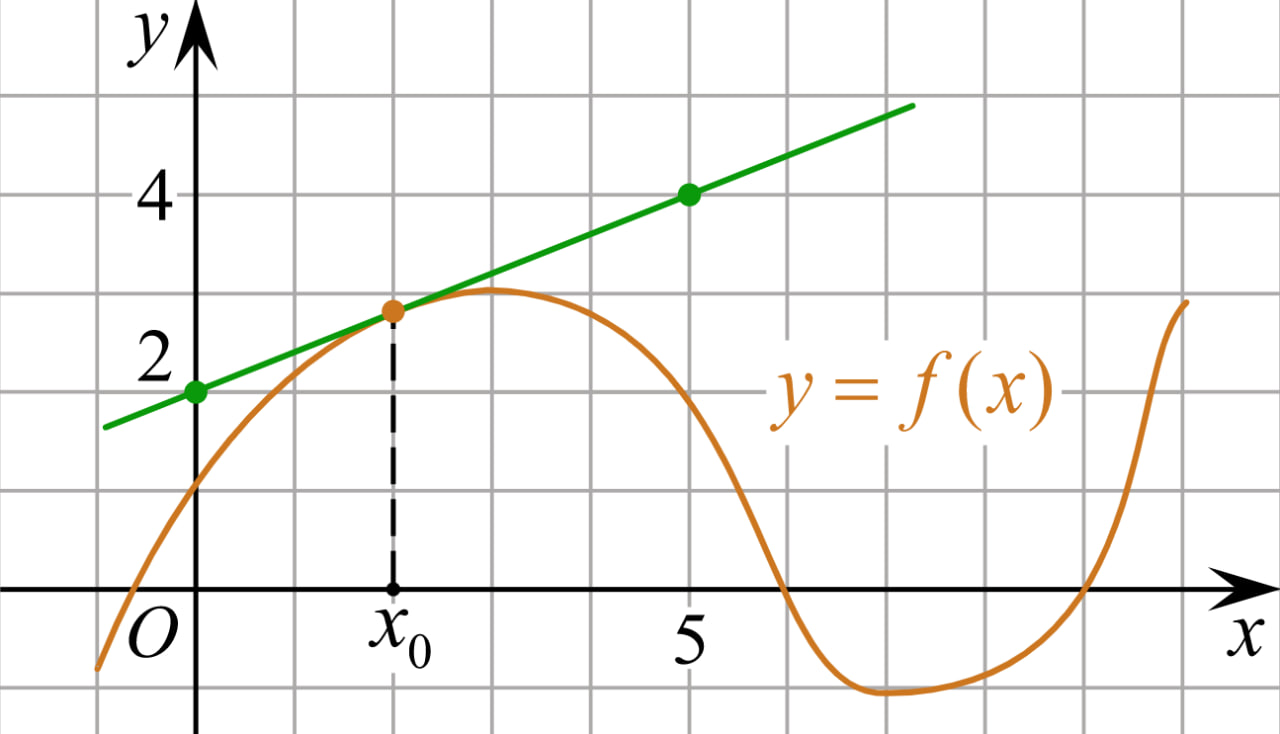
\includegraphics[align=t, width=\linewidth]{\picpath/G113M9H2}
		\end{minipage}
		\item Прямая \( y=7x-5 \) параллельна касательной к графику функции \( y=x^2+6x-8 \). Найдите абсциссу точки касания.
		\item Игорь и Паша красят забор за \( 9 \) часов. Паша и Володя красят этот же забор за \( 12 \) часов, а Володя и Игорь --- за \( 18 \) часов. За сколько часов мальчики покрасят забор, работая втроем?
		\item Найдите наименьшее значение функции \( y=2x^2-5x+\ln x-3 \) на отрезке \( \left[ \dfrac{5}{6}; \dfrac{7}{6} \right] \)
		\item \begin{tasks}(1)
			\task Решите уравнение: \( 2^{4\sin^2x+1}+2^{4\cos^2x}=18 \).
			\task Найдите все корни этого уравнения, принадлежащие отрезку \( \left[ 2\pi; \dfrac{7\pi}{2} \right] \).
		\end{tasks}
		\item Решите неравенство: \( \log_2(x^2+4x)+\log_{0,5}\dfrac{x}{4}+2\ge\log_2(x^2+3x-4)\).
		\item Решите неравенство: \( \log_x(x^3-8)\le\log_x(x^3+2x-13) \).
		\item \( 15 \)-го декабря планируется взять кредит в банке на сумму \( 300 \) тысяч рублей на \( 21 \) месяц. Условия возврата таковы:\\		
		--- \( 1 \)-го числа каждого месяца долг возрастает на \( 2\% \) по сравнению с концом предыдущего месяца;\\
		--- со \( 2 \)-го по \( 14 \)-е число каждого месяца необходимо выплатить часть долга;\\
		--- \( 15 \)-го числа каждого месяца с \( 1 \)-го по \( 20 \)-й долг должен быть на одну и ту же сумму меньше долга на \( 15 \)-е число предыдущего месяца;\\		
		--- \( 15 \)-го числа \( 20 \)-го месяца долг составит \( 100 \) тысяч рублей;\\
		--- к \( 15 \)-му числу \( 21 \)-го месяца кредит должен быть полностью погашен.\\
		Найдите общую сумму выплат после полного погашения кредита.
		\item Найдите все значения параметра \( a \) при каждом из которых уравнение
		\[x^2+a^2-2x-6a=|6x-2a|\]
		имеет ровно два различных корня.
>>>>>>> 8062ba7ed7664427492317023bec527c42abfc0f
	\end{listofex}
\end{homework}
%END_FOLD

%BEGIN_FOLD % ====>>_____ Занятие 5 _____<<====
\begin{class}[number=5]
	\begin{listofex}
<<<<<<< HEAD
		\item Занятие 5
=======
		\item 5
>>>>>>> d1e201b6c9252ede8c5810d54bc7e6ef776ad4a9
	\end{listofex}
\end{class}
%END_FOLD

%BEGIN_FOLD % ====>>_____ Занятие 6 _____<<====
\begin{class}[number=6]
	\begin{listofex}
<<<<<<< HEAD
		\item Занятие 6
=======
		\item 6
>>>>>>> d1e201b6c9252ede8c5810d54bc7e6ef776ad4a9
	\end{listofex}
\end{class}
%END_FOLD

%BEGIN_FOLD % ====>>_ Домашняя работа 3 _<<====
<<<<<<< HEAD
\begin{homework}[number=3]
	\begin{listofex}
<<<<<<< HEAD
		\item Домашняя работа 3
=======
\begin{homework}[number=2]
	\begin{listofex}
		\item 3
>>>>>>> d1e201b6c9252ede8c5810d54bc7e6ef776ad4a9
=======
		\item \( 31 \) декабря \( 2014 \) года Тимофей взял в банке \( 7 007 000  \) рублей в кредит под \( 20\% \) годовых. Схема выплаты кредита следующая: \( 31 \) декабря каждого следующего года банк начисляет проценты на оставшуюся сумму долга (то есть увеличивает долг на \( 20\% \)), затем Тимофей переводит в банк платёж. Весь долг Тимофей выплатил за \( 3 \) равных платежа. На сколько рублей меньше он бы отдал банку, если бы смог выплатить долг за \( 2 \) равных платежа?
		\item В июле планируется взять кредит на сумму \( 1 342 000 \) рублей. Условия его возврата таковы:\\
		--- каждый январь долг возрастает на \( 20\% \) по сравнению с концом предыдущего года;\\		
		--- с февраля по июнь каждого года необходимо выплатить некоторую часть долга.\\		
		На сколько рублей больше придётся отдать в случае, если кредит будет полностью погашен четырьмя равными платежами (то есть за \( 4 \) года), по сравнению со случаем, если кредит будет полностью погашен двумя равными платежами (то есть за \( 2 \) года)?
		\item В июле \( 2016 \) года планируется взять кредит в банке на четыре года в размере \( S \) млн рублей, где \( S \) --- целое число. Условия его возврата таковы:\\		
		--- каждый январь долг увеличивается на \( 15\% \) по сравнению с концом предыдущего года;\\		
		--- с февраля по июнь каждого года необходимо выплатить часть долга;\\		
		--- в июле каждого года долг должен составлять часть кредита в соответствии со следующей таблицей.
		\begin{table}[h]
			\begin{tabular}{llllll}
				\hline
				\multicolumn{1}{|c|}{Месяц и год}         & \multicolumn{1}{c|}{Июль 2016} & \multicolumn{1}{c|}{Июль 2017} & \multicolumn{1}{c|}{Июль 2018} & \multicolumn{1}{c|}{Июль 2019} & \multicolumn{1}{c|}{Июль 2020} \\ \hline
				\multicolumn{1}{|c|}{Долг (в млн рублей)} & \multicolumn{1}{c|}{S}         & \multicolumn{1}{c|}{0,8S}      & \multicolumn{1}{c|}{0,5S}      & \multicolumn{1}{c|}{0,1S}      & \multicolumn{1}{c|}{0}         \\ \hline
			\end{tabular}
		\end{table}
		Найдите наибольшее значение \( S \), при котором общая сумма выплат будет меньше \( 50 \) млн рублей.
>>>>>>> 8062ba7ed7664427492317023bec527c42abfc0f
	\end{listofex}
\end{homework}
%END_FOLD

%BEGIN_FOLD % ====>>_____ Занятие 7 _____<<====
\begin{class}[number=7]
<<<<<<< HEAD
	\title{Подготовка к проверочной}
	\begin{listofex}
		\item Занятие 7
=======
	\begin{listofex}
		\item 7
>>>>>>> d1e201b6c9252ede8c5810d54bc7e6ef776ad4a9
	\end{listofex}
\end{class}
%END_FOLD

<<<<<<< HEAD
%BEGIN_FOLD % ====>>_ Проверочная работа _<<====
\begin{exam}
	\begin{listofex}
		\item Проверочная
	\end{listofex}
\end{exam}
=======
%BEGIN_FOLD % ====>>_____ Занятие 8 _____<<====
\begin{class}[number=8]
	\begin{listofex}
		\item 8
	\end{listofex}
\end{class}
>>>>>>> d1e201b6c9252ede8c5810d54bc7e6ef776ad4a9
%END_FOLD